\chapter{Implementácia prostredia}
Prostredie bolo implementované v jazyku C++ vzhľadom na použité nástroje Flex a Bison. Kapitola je zameraná na použité štruktúry, vysvetlenie výberu týchto štruktúr a použité algoritmy.\\
V tej to kapitole sa používa nasledujúce značenie:
\begin{description}
\item[Kontext]\hfill \\
	Pojem kontext je v tejto kapitole používaný sa definovaie relevantých okolností, za akých je vykonávaná inštrukcia kódu. Zjednodušene povedané, popis toho, akou najkratšou cestou, myslené vykonávaním kódu, je možné dostať sa k vykonávaniu danej inštrukcie, pričom relevatné sú iba volania funkcií a definovanie nových blokov. Matematicky povedané, kontext je usporiadaný zoznam volaní funkcií a definoaní nových blokov. Príkladom: nech máme kód tak, ako je naznačený v tabuľke \ref{tab:rek}, potom kontext inštrukcie zodpovedajúcej riadku 3 je <main(),f(),\{>. Napriek tomu, že funkcia f je rekurzívna a hĺbka zanorenia môže byť iná. Z opačného pohľadu, v rovnakom kontexte sa môžu vyskytovať viaceré inštrukcie. V našom príklade je tomu tak pri volaní funkcie f na riadku 4. kontext volania  funkcie f na riadku 8 je <main()>
\item[Premenná] \hfill \\
	Pojem premenná reprezentuje dáta pomenované jednoznačným reťazcom začínajúcim písmenom alebo podtržítkom. Napríklad \it{integer test} je premenná s názvom test, ktorá je typu integer. Slovo test by v danom kontexte nemalo byť použité pre inú premennú. V tabuľke \ref{tab:rek} je teda premenná a zadefinovaná chybne, pretože existujú dve premenné a v rovnakom kontexte.
\item[Premenné robota]\hfill \\
Premenná robota je taká premenná, o ktorej robot predpokladá, že data v nej sa menia len v závislosti na jeho akciách. Predpokladajme, že v tabuľke \ref{tab:rek} je definovaný kód robota A. Potom a je premenná robota A. Pokiaľ existuje iný robot B, nemá žiaden vplyv na premennú a robota A.
\item [Tick] \hfill \\
	označuje je jednotka virtuálneho času sveta. počet tikov, koľko trvá jedno kolo, je záväznú pre všetkých robotov a závisí na plánovači. Defaulte sa jedn tick rovná jedno kolo.
\item[Penalizácia za inštrukciu]
	je počet tikov, ktoré robot stratí, ak inštrukciu vykoná. Pre rôzne inštrukcie môže byť (a typicky bude)rôzna.
\item [Program robota] 
	značí postupnosť inštrukcií
\item [ProgramPointer]
 	je ukazateľ na inštrukciu v programe. Druhy inštrukcií a ich vplyv na svet je popísaný v \ref{instrukcie}.
\end{description}

\begin{table}
\centering
\begin{tabular}{| lll |}
\hline
1&void function f()\\
2&\{\\
3&&integer a;\\
4&&f();\\
5&&integer a;\\
6&\}\\
7&int main()\\
\{\\
8&&	f();\\
9&\}\\
\hline
\end{tabular}
\caption{ Príklad kódu robota }
\label{tab:rek}
\end{table}

Každý robot má vlastný program, užívateľom definovaný, podľa ktorého sa správa. Tento program sa z hľadiska jednotlivého robota skladá z postupnosti základných inštrukcií, ktoré sú ďalej nedeliteľné. 

\section{Priebeh penalizácie za inštrukciu}

\begin{definicia}
\end{definicia}

Nech je na rade robot R. R sa pozrie, či už ubehla dostatočne dlhá doba od vykonania jeho poslednej akcie. Ak áno, R začne vykonávať inštrukciu, na ktorú práve ukazuje jeho ProgramPointer. Po vykonaní tejto inštrukcie si poznamená, koľko ho stála tickov. Ak ešte neprebehla dostatočne dlhá doba, potom počká a na rade je ďalší objekt. \\
Penalizácia prebieha podľa aktuálnej tabuľky penalizácií, ako bola nastavená v základnom menu. \\

Týmto spôsobom sa efektívne vyrieši prípad, kedy robot premýšľa príliš dlho alebo keby sa zacyklil. Keďze po každej vykonanej inštrukcii predá riadenie daľšiemu objektu, zacyklenie sa pozná len podľa toho, že robot sa nebude hýbať, ale nijak to nespomalí ostatné objekty.%TODO ref
\newline
Nech je na rade objekt rôzny of typu 'robot'. Potom tento objekt má konštantnú penalizáciu (strela štandartne 0) a jeho program obsahuje iba inštrukcie, ktoré interagujú s bojiskom.Sú rôzne v závislosti na type objektu.

\subsection{Poradie vykonávaných akcií}

Rozhodovanie robota, či má vykonať inštrukciu, prebieha tým spôsobom, že sa podľa tabuľky \ref{penal} spočíta, koľko času robot prehmrhal na myslenie, a podla toho sa robot N-krát robot sa vzdá vykonania inštrukcie, kde N sa dá vypočítať dvoma spôsobmi.\\
N sa bude rovnať penalizácií za jednu, inštrukciu a teda presne toľkokrát príde robot na radu a nebude robiť nič, len predá slovo ďalšiemu objektu. Výhodou je, že tento prístup je pomerne priamočiary, ľahko implementovateľný. Nevýhodou tohoto prístupu je, že zatiaľ čo pohyb objektov musí byť vykrelovaný v závislosti na čase, aby sa predišlo závislosti na rýchlosti procesora a táto penalizácia nie, výsledok je, že robot sa pohne alebo otoči, poťažne vystrelí a potom najmenej 3 kolá musí stáť ( load premennej, load konstanty a uloženie), pričom za ten čas povedzme strely môžu uraziť príliš veľký kus a robot na ne nemá sancu zaregovať.\\
Ďalšou možnosťou je podobne ako pri vykresľovaní pohybu striel a stien sa aj k ostatným inštrukciám správať ako na závislé na čase. Penalizácie ako sú popísané v tabuľke \ref{penal} nebudú značiť priamo čas, ale akú časť z pevne daného množstva F zaberajú. Za predpokladu, že posledný čas aktualizovania(odvtedy, čo vykonal nejakú inštrukciu) robota bol T, aktuálny čas je TA, potom robot vykoná inštrukciu, vypočíta si jej čas, ktorý zaberá = F/penalize(instruction) a bude vykonávať inštrukcie tak dlho, pokiaľ suma týchto vypočítaných inštrukcií nebude väčšia nanajvýš rovná rozdielu medzi aktuálnym časom a časom posledného aktualizovania. V pseudokóde to vyzerá približne takto:\\
$ Uint32 diff= actualTime - timeLastUpdate;\\ while (diff > 0)\\\{\\ diff-=nextInstruction.penalize();\\nextInstruction.run();\\Pointer ++; \\\}\\ $ Tento spôsob je viac šetrnejší k robotovi,pozastai objekty, aby na ne mohol robot reagovať, čo je v simulácií ako Codewars podstatné.	

\section{Hracia plocha} % z coho sa sklada
Na začiatku hry sa vygeneruje mapa s veľkosťou, ktorú zadá užívateľ, alebo sa načíta už uložená mapa. Táto pozostáva zo voľných políčok a stien. Steny sú rôzneho typu, viz \ref{walls}. Ďalej celú túto konštrukciu nazývam bojisko. V tomto okamihu je hra pripravená na spustenie. V závislosti na veľkosti bojiska sa čaká na odpovedajúce množštvo robotov, ktorí sa zapoja do hry. Toto množstvo je defaultne obmedzené iba zdola. Na zdôvodnenie tohoto rozhodnutia je nutné spomenúť základné vlastnosti programu. 
\subsection{Generovanie map}% ako sa generuje, podpora ukladania, zadne zhluky, vyhody, nevyhody, 
Jedným z užívateľsky príjemných vlastností aplikácie je aj možnosť vytvoriť si vlastné mapy. Pre tento účel je v aplikácií naimplementované samostatný editor, kde si môže užívateľ defnovať vlastnú mapu.
\section{Jazyk hry a priebeh hry} %bison, prec
\begin{definicia}
Cieľom určenia robota nazývam políčko na mape sveta, kam sa má robot dostať. Teda ak je pozícia robota rovnaká ako pozícia tohoto cieľa, hra končí. Týchto cieľov môže byť viac.  Pod vzdialenosťou rozumiem veľkosť obsahu obdĺžnika v vrcholmi cieľom a výskytom robota. %TODO preco?
\end{definicia}

Samotná hra prebieha tak, že roboti vykonávajú užívateľom definovaný kód až do okamžiku, keď dosiahnu víťazný stav alebo kým nezostane na bojisku maximálne jeden robot. Cieľ môže byť pre každého robota rozdielny a je jeho súčasťou. Hra nie je zabezpečená proti nekonečne dlhotrvajúcim cyklom (napríklad keď každý robot stojí na mieste), predpokladá sa v tomto prípade vstup od uživateľa, ktorým hru preruší.

\begin{definicia}
Stav robota vzhľadom na svet charakterizuje štvorica: (InstructionPointer IP, Hitpoints HP, VisualMemory vm, Direction direct), kde 
\begin{itemize}
\item InstructionPointer je odkaz do štruktúry programu robota hovoriaci, ktorá inštrukcia je na rade
\item HP je nezáporné celé číslo popisujúce životnosť robota
\item VirtualMemory je štruktúra obsahujúca objekty v zornom poli od posledného volania funkcie 'see()', volanej bez parametrov 
\end{itemize}
Stav robota s ohľadom na inštrukcie, ktore vykonáva, charakterizuje (PointerStack PS, ValueStack VS, Memory m) kde
\begin{itemize}
\item PS zoznam pointerov do štruktúry programu
\item VS je zásobník všetkých naloadovaných hodnôt, parametrov  a návratových adries z funkcií
\item Memory je zoznam všetký doteraz definovaných premenných a funkcií
\end{itemize}
\label{StavRobota}
\end{definicia}

\begin{definicia} 
Pod objektami sveta rozumieme všetky prvky, ktoré svet tvoria a zároveň ho z času na čas menia, t.j. v tomto prípade strely, steny, a samotní roboti. Napríklad strela mení svet tým, že sa pohne alebo narazí, istý druh steny sa môže posunúť a pod.
\end{definicia}
Svet je charakterizovaný dvojicou $< ZoznamObjektov, Bojisko >$, kde ZoznamObjektov obsahuje objekty, ktoré sú na rade, aby vykonali nejakú inštrukciu. Presný spôsob vykonávania inštrukcií je popísaný v \ref{schedulle} Objekty v tomto zozname sa počas priebehu boja menia, napríklad pribúdajú a zanikajú strely, ktoré sú podla \ref{defobjekty} tiež objektami, tiež môžu ubúdať steny ( niektoré majú svoju životnosť a dajú sa rozbiť ). \\

Pre všetky nasledujúc inštrukcie interagujúce so svetom predpokladajme, že svet je v stave $<ZoznamObjektov, Bojisko>$, kde ZoznamObjektov je postupnosť objektov $(robot X, objekt1, objekt2, objekt3,...objektN)$ a Bojisko je dvojrozmerná matica popisujúca, aké objekty sú na akých pozíciach.
Popis jednotlivých inštrukcií a ich vplyv na svet je symbolicky popísaný takto: (bez parameterov, ktoré nemajú vplyv na svet):\\
\newline
step:\begin {itemize}
\item Svet:$ < ObjectsList, m.reinsert(X) > $
\item Bot: $ < NewIP, Hp, direct> $
\end {itemize}
turnLeft, turnRight \begin{itemize}
\item $Svet:  <ObjectList, m>$
\item $Bot:  < NewIP, Hp, NewDirect)>$
\end{itemize}
turn  \begin{itemize}
\item $Svet:  < ObjectsList, m > $
\item $Bot:   < NewIP, Hp, NewDirect)> $
\end {itemize}
see  \begin{itemize}
\item $Svet:  <ObjectsList,m> $
\item $ Bot:  < NewIP, Hp, NewDirect)> $
\end {itemize}
shoot \begin {itemize}
\item $ Svet:  < AddedObjectsList, m> $ 
\item $ Bot:  < NewIP, Hp, Direct)>  $
\end {itemize}
\indent
kde ObjectsList je \\ $(Objekt_1, Objekt_2, ..., Objekt_K, X, Objekt_{k+1},.., Objekt_N)$, NewIP je nový ukazateľ do programu robota, nie nutne odlišný od predošlého(je možné zastať napríklad pri forcukle zastať na rovnakej inštrukcií), NewDirect je číslo 1-4 označujúce aktuálne natočenie robota, reinsert je funkcia, ktorá sa pokúsi robotom pohnut v mape, ak sa nedá vyvolá sa ošetrenie kolízií a AddedObjectList je\\ $(Objekt_1, Objekt_2, ... Objekt_N, Object_{strela})$ Strela sa vždy pridá na koniec zoznamu. Tým je zaručené, že roboti budú vedieť reagovať na strelu a porípade sa jej vyhnúť. %TODO rozviest
Ďalšie inštrukcie vôbec nekomunikujú so svetom, preto sú uvedené oddelene. Tieto inštrukcie robot vykonáva počas svojho premýšľania po skupinách podľa toho, ako moc času ubehlo. Keďze tým robot vôbec nepotrebuje vedieť o objektoch sveta iných než je on sám, po prevedení takýchto inštrukcií sa meni stav robota podla tabuľky \ref{VnutroBota},kde IP+1 znamená posun v atuálneho pointera v programe robota o jednu inštrukciu ďalej, AddedIP je uloženie aktuálneho pointera na inštrukciu a vyhlásenie iného pointera za aktuálny (typicky začiatok pricedúry alebo funkcie), VariablesAdded je pamať robota rozrastená o premenné danej funkcie alebo procedúry v danom zanorení, ClearVariables je označenie premennych definovaných v tomto bloku za neplatné, LoadByName je uloženie hodnoty volanej premennej na ValueStack, AddedResult je uloženie výsledku aritmetických operácií na ValueStack a DeleteIP je zrušenie aktuálneho pointera na funkciu a obnovenie predchádzajúceho na inštrukiu, pre ktrou bol prerušený. RemoveValue je spracovanie hodnoty zo ValueStacku a teda jej odobranie a odobranie premennej, do ktorej sa priradzuje.

\begin{table}[ht]
\centering
\caption{Vnutorné príkazy robota}
\begin{tabular}{|l|p{5cm}|}
\hline\hline
Inštrukcia & Stav bota po inštrukcii \\
store & $ IP+1,RemoveParameters$\\
aritmeticke+relacne operácie & $IP+1,AddedResult,m$ \\
Call &  $ AddedIP,VS,VariablesAdded$\\
StartBlock & $IP+1,VS,m$\\
EndBlock & $IP+1,VS,ClearVariables$\\
Load & $ IP+1,LoadByName,m$\\
Label & $ IP+1,VS,m$\\
Jump & $ DeleteIP,VS,t$\\
\hline
\end{tabular}
\label{VnutroBota}
\end{table}
\subsection{Priebeh výpočtu robota} %co je povolene a ako sa to riesi implementacne
TODO
Jazyk pre Codewars je rozpoznavaný pomocou nástrojov Flex pre lexikálne rozpoznávanie a Bison pre syntaktické. Keďze Flex vyžaduje pre lexikálne rozpoznávanie v podstate len súbor tvorený regulárnymi výrazmi a konštantami pre detekciu tokenov a Bison iba súbor s definíciami gramatiku a pomocnými štruktúrami, je tento spôsob veľmi priehľadný, ľahko udržovateľný a modifikovateľný, preto bol zvolený. Následuje popis štruktúr  a popis práce s nimi:
\begin{huge}TODO \end{huge}
\\
Zaujímavejšie je to pri volaní funkcie, ktorá má defaultný parameter. Pretože sa predpokladá, že program bude prístupný aj pre obyčaných užívateľov, je možné u funkcie definovať aj explicitnú hodnotu a to nezávisle na poradí parametrov. T.j. explicitné hodnota môže byť zadaná ako prvý a tretí parameter, ale nie ako druhý. Takáto funkcia sa nadefinuje podobne ako v C/C++, napríklad : \\\begin{center} $ function distance(integer x=3, integer y=2, integer radius, Location l) $ \\\end{center}V okamžiku, keď sa zavolá \begin{center} $ distance(, , radius,l) $ \end{center} sa ušetrí loadovane dvoch premenných.

\subsection{Zaujímave nastavenia a efekty}

Velmi špeciálny je prípad, keď užívateľ nenastaví robotovi žiadnu pamäť. Takýto robot nie je schopný si zapatať jedinú premennú a ani vracat návratové hodnoty, teda v kóde programu by nemali byť definované žiadne funkcie, ale iba procedúry.Je nutné povedať, že funkcie a procedúry sa v žiadnom prípade nechovajú ako premenné a teda nezaberajú robotovi pamať. Teda v tomto prípade dojde k masívnemu využitiu rekurzií. Samotne vstavané príkazy sú však vlastne funkcie, ale kedže sa nikam nemajú priradiť, ich návratová hodnota sa zahodí. Nevýhodou tohoto typu bota je však skutočnost, že  nepríklad strieľať alebo pohybovať sa môže len pomocou konštaty. Iné hodnoty nemajú garantované miesto v pamäti

\subsection{Zrak robota}
Vo vstupe si užívateľ má možnosť nastavit premennú, ktorá ovplyvňuje to, ako ďaleko bude robot vidieť do strán. Je to premenná $\alpha$, ktorá označuje uhol, pod ktorým vidí robot na jedno oko. Pochopiteľne má robot symetrické oči a teda do druhej strany vidí pod rovnakým uhlom. Jedným z pomerne rýchlych spôsobov, ako určiť viditeľné objekty, je následuuci algoritmus:

\begin{figure}
\centering
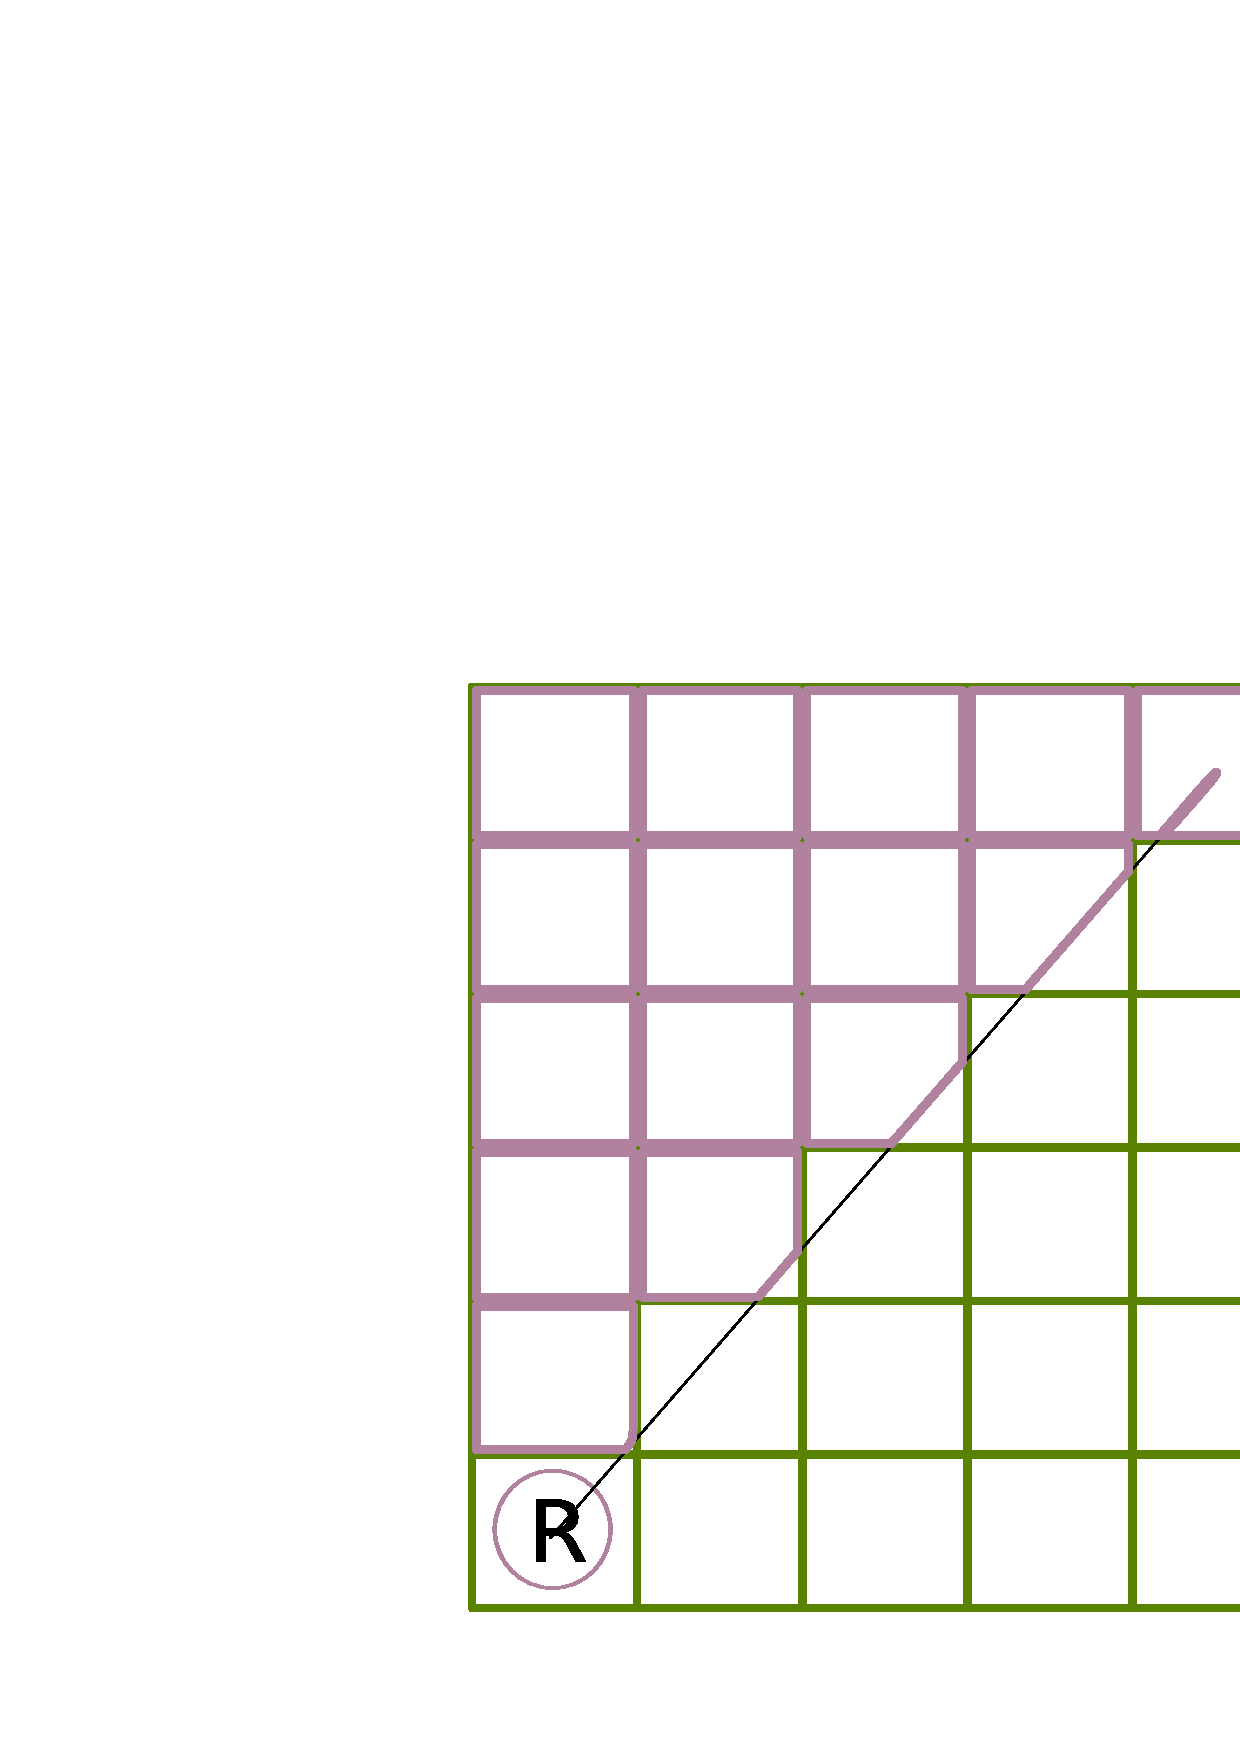
\includegraphics[totalheight=0.2\textheight,width=.6\textwidth]{chooseVisible}
\caption {Výber parametrov pre zrak robota}
\label{choosing}
\end{figure}

\begin{definicia}
Pod zorným poľom robota rozumieme hornú polovicu trojuholníka určeného uhlopriečkou medzi vrcholmi obdĺžnika o veľkosti X,Y. Robot vidí objekt v okamihu, ked vidí stred políčka, na ktorom objekt stojí a úsečka spájajúca tieto dva body nepretína žiadny ďalší blokujúci objekt. blokujúci objekt je definovaný implementáciou, v našom prípade je blokujúci objekt robot a stena, neblokujúci strela. toto rozdelenie vychádza z bežneho pozorovania, že drobná stela nemá tendenciu zakrývať výhľad.
\end{definicia}
Obdĺžnik môže mať vzhľadom na implementáciu maximálne obsah 32, čo je na väčšine architektúrách veľkosť integeru. Toto číslo bolo zvolené, pretože je dostatočne veľké a súčasne vysoko dostupné na rôznych architektúrach. Samotne detekovanie toho, čo robot vidí, prebieha nasledujúco: \\
\begin{figure}
\centering
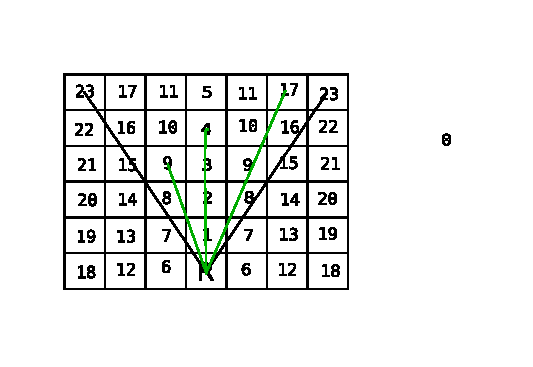
\includegraphics[totalheight=0.4\textheight,width=.8\textwidth]{visibility}
\caption {Viditeľnosť robota s parametrom uhla $20_\circ$}
\label{visibility}
\end{figure}
Nech má obdĺžnik rozmery (x,y) a jeho dolný ľavý vrchol je na pozícií (0,0), čo je v podstate pozícia bota. Obdĺžnik je teda rozdelený na XxY menších obdĺžničkov. Kazdý z nich má svoje poradové číslo a masku, ktorá má na i-tej pozícií jedničku práve vtedy, ak úsećka počínajúca v bode [0.5,0.5],čo je stred políčko s robotom, a stredom skúmaného políčka prechádza políčkom s identifikaćným číslom ID. takto ale robot bude vidieť len na jednu stranu, ale keďže druhá polovička je presne symetrická, môžeme tieto práve vygenerované masky použiť, viz \ref{visibility}  na obe strany bez upravovania. \\
Podla obrázka \ref{visibility} bude mať políčko s ID 4 masku 1111, pretože na to, aby ho bolo vidno, je nutné vidieť políčka s ID 1,2,3. Podobne políčko 9 bude mať masku 110000011, pretože úsečka spájajúca tieto dva body prebieha tiež týmito políčkami. Zistenie, či práve toto políčko je pretnuté úsečkou, sa takto zjednodušuje na nájdenie všeobecnej rovnice priamky s koncovými bodmi v stredoch týchto dvoch políčoka zistenie, či pravý dolný vrchol a ľavý horný vrchol patria rovnakej polrovine generovanej touto priamkou.\\
obdĺžnik, podľa ktorého sa zrak ďalej určí.
Za života robota sa jeho zrak nemení a teda môžeme použiť tieto vygenerované masky bez ďalšieho prepočítavania. Pri volaní metody see(), ktorá dodá viditeľné objekty robotovi, potom stačí namapovať náš obdĺžnik na príslušné miesto na mape(podľa robotovej pozície a natočenia), nastaviť 1 na i-té miesto políčka s ID = i, na ktorom nie je nič alebo len neblokujúci objekt, a výslednú masku porovnať s predtým vypočítanou maskou každého políčka, na ktoré by robot mohol vidieť. Nech zisťujeme, či vidíme objekt na pozícií na mape X,Y, ktorý sme namapovali na políčko s ID = I a maskou M. Ak výsledná maska má jedničky presne na tých istých miestach ako M, potom I je viditeľné, pretože všetky políčka, na ktorých I záviselo, boli označené ako viditeľné. \\
Nech existuje také políčko s ID = P, na ktorom je nejaký blokujúci objekt. Potom vo výslednej maske bude na P-tom mieste 0 a políčko I, ak úsečka spájajúca stredy políčok robota a I prechádzala cez P, bude mať na P-tom mieste 1. Maska políčka I bude mať teda o minimálne jednu 1 viac ako výsledná maska a teda políčko bude označené ako neviditeľné.\\
Na obrázku \ref{visibleo} je červeným znázornen=y objekt, ktorý robot uź neuvidía zelenou, ktorý uvidí. Napríklad je viditeľný robot R, pretože pred ním je strela S a keďže je neblokujúca, políčko 4 pripojilo na výslednej maske 1 na 4.pozícií. Pozícia 5 má masku 1111 a teda je viditeľná.

\begin{figure}
\centering
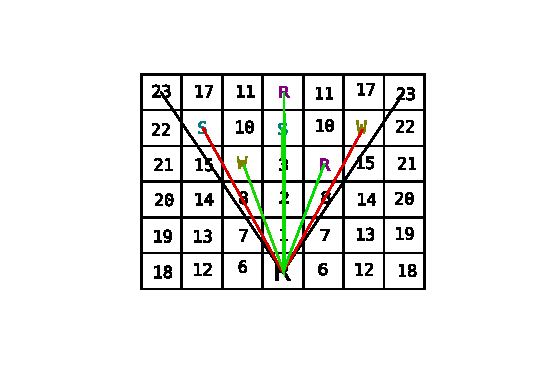
\includegraphics[totalheight=0.4\textheight,width=.8\textwidth]{VisibleObjects}
\caption { Objekty v zornom poli robota}
\label{fig:visibleo}
\end{figure}
\indent
\newline
\indent Tento spôsob má ale nevýhodu pri použití v programoch typu Codewars. Predpokladá totiž, že v okamžiku žiadosti o naplnenie viditeľných ojektov budú tieto objekty stáť presne v strede daných políčok. Ak by povedzme jedna stena stála presne nedzi dvoma políčkami, už nie jasné, aké políčka robot vidí. Preto bol primo v implementácií použitý spôsob porovnania uhlov viditeľnosti.
\\
\begin{figure}
\centering
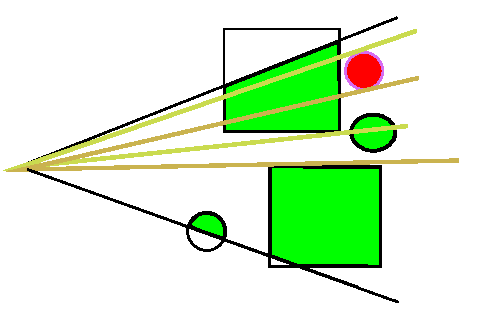
\includegraphics{visibility2}
\caption { Objekty v zornom poli robota podľa fruhého algortimtmu. červeným je vyznačený objekt, ktoré nie je vidno}
\label{fig:visibleo}
\end{figure}
\indent
